\documentclass{beamer}
\usetheme{Madrid}

\title{Control Systems (EE2227) Presentation}
\author{Sudeep Veggalam \\ EE18BTECH11045}
\centering
\date{12 February 2019}
\begin{document}
\maketitle
\begin{frame}{Problem Statement}
\framesubtitle{GATE 2017 (Set II) Question 26}
    \begin{block}{Question}
        \item Which of the following systems has maximum peak overshoot due to a unit step input?
     \end{block}
\begin{itemize}
    \item(A) $100 / s^2 + 10s + 100$
    \item(B) $100 / s^2 + 15s + 100$
    \item(C) $100 / s^2 + 5s + 100$
    \item(D) $100 / s^2 + 20s + 100$
\end{itemize}
\end{frame}
\begin{frame}{Theory}
The transfer function for the second order control system is given by:
\begin{equation}
    \dfrac{C(s)}{R(s)}= \dfrac{\omega_n^2}{s^2 + 2\zeta\omega_ns + \omega_n^2}
\end{equation}
To calculate the unit step response,
\\$r(t) = 1$ or $R(s) = \dfrac{1}{s}$
\\On Simplifying, 
\begin{equation}
    C(s) = \dfrac{1}{s} - \dfrac{s + \zeta\omega_n}{(s + \zeta\omega_n)^2 + \omega_d^2} - \dfrac{\zeta\omega_n}{\omega_d}.\dfrac{\omega_d}{(s + \zeta\omega_n)^2 + \omega_d^2}  
\end{equation}
\\where,
\\$\omega_d=\omega_n\sqrt{1-\zeta^2}$
\\This is the Unit step response in frequency domain
\end{frame}
\begin{frame}{Theory (contd.)}
    Take inverse laplace transform to get the unit step response in time domain:
\begin{equation}
    c(t) = 1 - e^-\zeta\omega_nt(cos\omega_dt+\dfrac{\zeta}{\sqrt{1-\zeta^2}}.sin\omega_dt)
\end{equation}
\\This is the time domain representation of unit step response
\end{frame}
\begin{frame}{Theory (contd.)}
    \begin{block}{What is Peak overshoot?}
        \item \textbf{Maximum overshoot} is the difference between the magnitude of the highest peak of time response and magnitude in its steady state. Peak Overshoot is expressed in term of percentage of steady-state value of the response.
        \begin{equation}
            M_p = \dfrac{c(t_p) - c(\infty)}{c(\infty)} * 100 \%
        \end{equation}
     \end{block}
\end{frame}
\begin{frame}{Peak Overshoot}
Mathematical expression for Peak Overshoot:
\\c(t) is max where $\dfrac{dc(\emph{t})}{d(\emph{t})}$
\\On applying this condition on (3), we get
\begin{equation}
    t_p = \dfrac{\pi}{\omega_n\sqrt{1-\zeta^2}}
\end{equation}
\\Substituting in the equation for Peak overshoot:
\begin{equation}
    M_p = e^\dfrac{-\zeta\pi}{\sqrt{1-\zeta^2}}
\end{equation}
\end{frame}
\begin{frame}{Solution}
    \begin{flushleft}
    From (6), we can infer that Peak Overshoot is a decreasing function of $\zeta$
    \\i.e The second order equation with the lowest $\zeta$ will have the maximum peak overshoot
    \\For option (A), $\zeta = 0.5$
    \\For option (B), $\zeta = 0.75$
    \\For option (C), $\zeta = 0.25$
    \\For option (D), $\zeta = 1$
    \\Therefore, (C) has the maximum peak overshoot
    \\Answer : (C)
    \end{flushleft}
\end{frame}

\begin{frame}{Plotting}
\begin{columns}[t]
\column{.5\textwidth}
\centering
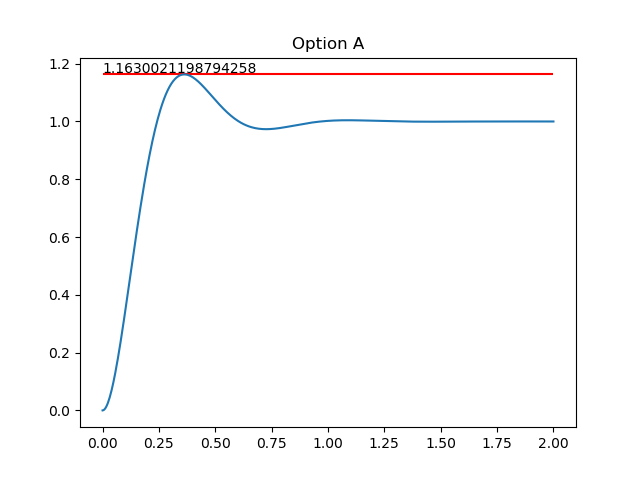
\includegraphics[width=5cm,height=4cm]{optionA.png}\\
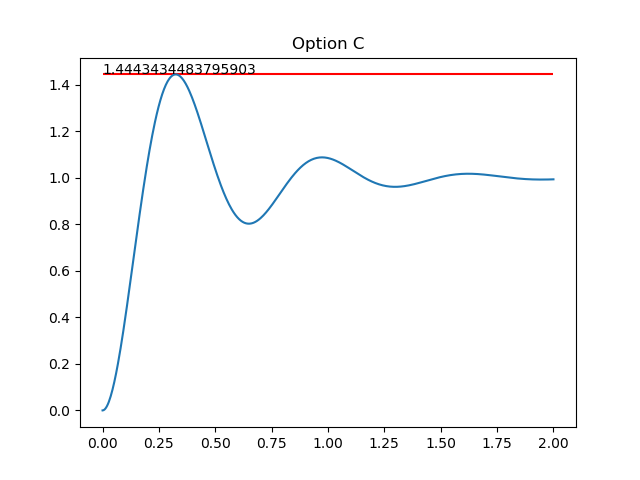
\includegraphics[width=5cm,height=4cm]{optionC.png}
\column{.5\textwidth}
\centering
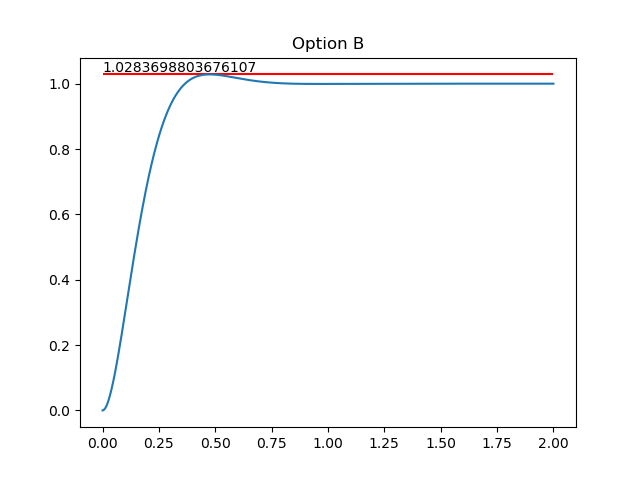
\includegraphics[width=5cm,height=4cm]{optionB.png}\\
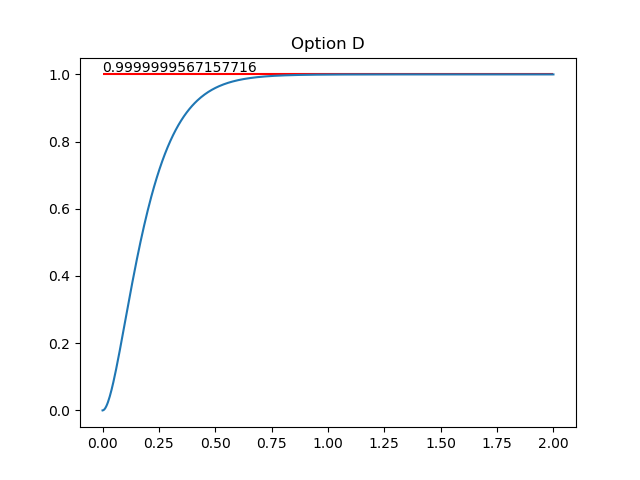
\includegraphics[width=5cm,height=4cm]{optionD.png}
\end{columns}
\end{frame}

\end{document}
